\documentclass[conference]{IEEEtran}
\IEEEoverridecommandlockouts
% The preceding line is only needed to identify funding in the first footnote. If that is unneeded, please comment it out.
\usepackage{cite}
\usepackage{amsmath,amssymb,amsfonts}
\usepackage{algorithmic}
\usepackage{graphicx}
\usepackage{textcomp}
\usepackage{xcolor}
\usepackage{tikz}
\usetikzlibrary{calc}
\def\BibTeX{{\rm B\kern-.05em{\sc i\kern-.025em b}\kern-.08em
    T\kern-.1667em\lower.7ex\hbox{E}\kern-.125emX}}
\begin{document}

\title{A system to analyse hygiene and to perform an automatic cleaning of public lavatories\\
{%\footnotesize \textsuperscript{*}Note: Sub-titles are not captured in Xplore and
%should not be used
}
%\thanks{Identify applicable funding agency here. If none, delete this.}
}
\author{
    \IEEEauthorblockN{1\textsuperscript{st} Fathima B}
    \IEEEauthorblockA{\textit{Department of Computer Application}\\
    \textit{College of Engineering Trivandrum}\\
    Trivandrum, India\\
    fathimabadar008@gmail.com}\\
    
    \IEEEauthorblockN{3\textsuperscript{rd }Atheana M S }
    \IEEEauthorblockA{\textit{Department of Electrical and Electronics Engineering} \\
    \textit{College of Engineering Trivandrum}\\
    Trivandrum, India\\
    atheana.m.s@gmail.com}
    \and
    
    \IEEEauthorblockN{2\textsuperscript{nd} Sashwat K }
    \IEEEauthorblockA{\textit{Department of Computer Application} \\
    \textit{College of Engineering Trivandrum}\\
    Trivandrum, India\\
    sashwat@cet.ac.in}\\
    
    \IEEEauthorblockN{4\textsuperscript{th} Rithwik Rajeev M }
    \IEEEauthorblockA{\textit{Department of Computer Science and Engineering} \\
    \textit{College of Engineering Trivandrum}\\
    Trivandrum, India\\
    rithwikrtk@gmail.com}
    }
\maketitle

\begin{abstract}
In India, we have a sufficient number of public toilets (including train toilets), but people hesitate to use it due to lack of cleanliness. The proposed system ensures the hygiene of public lavatories (including train toilets) after every use and prepares it for the next use. The system analyses the cleanliness of the toilet after one's usage, and based on the analysis it can perform a basic cleaning automatically to maintain the hygiene standards for the next use. The system uses affordable and reliable electronic devices for analysing and automating cleaning processes.

\end{abstract}
\begin{IEEEkeywords}
hygiene, IR, odour, sensors, solenoid, raster scan, MQ-136, MQ-137
\end{IEEEkeywords}

\section{Introduction}
Public toilets and latrine systems are maintained clean by janitors. Even though they are cleaned regularly, people tend to leave them dirty or by frequent use, it turns dirty. This not only keeps people away from using public lavatories but also using it under unhygienic condition causes health issues.  The inadequate domestic and personal hygiene leads to diseases like food poisoning, gastroenteritis, diarrhoea, pneumonia and skin infections.  Many times people, especially ladies and kids, hesitate to use public toilets due to the unhygienic conditions. This gives rise to abnormal health conditions like urinary infections, kidney stones and other illness.

The proposed system is aimed at maintaining hygienic standards in public latrines and toilets by automatically pre-cleaning them. It is to be noted that the mechanism doesn't include advance cleaning of the toilet but prepares for temporary and urgent use. It minimises the workload of janitors and provides a better hygienic working environment. The system works as follows
\begin{itemize}

\item When a person leaves the toilet after his/her use, the analysing process gets initiated
    \begin{itemize}
 
      \item The IR camera will search for solid wastes in the toilet bowl.
      \item Similarly, it will search for dirt, mud and other particles on the floor.
      \item Gas sensor checks the development of sulphur and ammonium derived gases which causes a foul smell.
    \end{itemize}{}
\item Based on the analysis, if the system warns that the toilet is unhygienic to use, an automatic basic cleaning process gets initiated.
    \begin{itemize}
    \item An automatic flush controlled by a solenoid valve to clean the toilet bowl.
    \item An automatic air freshener gets activated if there is any presence of foul-smelling gases. These gases are detected using gas sensors present in the system.
    \item A custom mechanism is used to clean the dirt and mud on the floor. It consists of custom mechanical brush with a flexible hose supplying water at the middle. The custom brush raster scans to cover almost all parts of the floor. A custom hose is used to spray at high pressure to clean the areas where the brush cannot reach.
    \end{itemize}{}
\end{itemize}

Other components include LEDs, LDR sensors and indicator buttons. The LEDs corresponds to indicator buttons, which are fixed outside the toilet door. These indicators conveys to the user whether the toilet is hygiene to use or it is under processing or if an advance cleaning is required. The system doesn't perform cleaning process unless it is required and it does not perform all the modules in the process, rather it only performs the modules that which are necessay. The system uses these techniques to raise the standard of public hygiene in most economic and energy efficient manner possible.

\section{Related Works}
    The idea of automatic cleaning of toilets has many parallels now. Among that, E-toilets are most popular and prominent one. But this system is entirely different from E-toilets in the aspect of technology used, objectives and many more. It is used in places where there is no proper facility for public sanitation and has limitation to construct public toilets due to lack of space. The E-toilets has been implemented in highly populated cities. It uses high-pressure vacuum for cleaning and it is completely automatic. No manual cleaning is required. The cost of implementing one E-toilet will range from 2 to 5 lakhs. But, E-toilet doesn't solve the hygiene issue of already existing public toilets. And now most of the E-toilets are under maintenance condition due to the failure of system components.
    Similarly, many other parallels are now available. But most of them require a new toilet design for implementing.

\section{Block Diagram}
    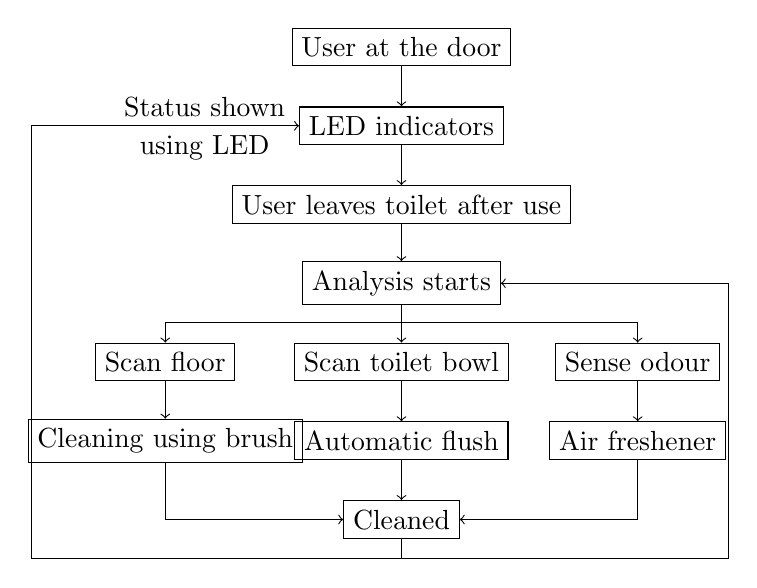
\begin{tikzpicture}
    \node[draw] (v1) at (3,0) {User at the door};
    \node[draw] (v2) at (3,-1) {LED indicators};
    \node[draw] (v3) at (3,-2) {User leaves toilet after use};
    \node[draw] (v4) at (3,-3) {Analysis starts};
    \node[draw] (v5) at (0,-4) {Scan floor};
    \node[draw] (v6) at (3,-4) {Scan toilet bowl};
    \node[draw] (v7) at (6,-4) {Sense odour};
    \node[draw] (v8) at (0,-5) {Cleaning using brush};
    \node[draw] (v9) at (3,-5) {Automatic flush};
    \node[draw] (v10) at (6,-5) {Air freshener};
    \node[draw] (v11) at (3,-6) {Cleaned};
    
    \draw[->] (v1) -- (v2);
    \draw[->] (v2) -- (v3);
    \draw[->] (v3) -- (v4);
    \draw[->] (v4) -- (3,-3.5) -- (0,-3.5) -- (v5);
    \draw[->] (v4) -- (v6);
    \draw[->] (v4) -- (3,-3.5) -- (6,-3.5) -- (v7);
    \draw[->] (v5) -- (v8);
    \draw[->] (v6) -- (v9);
    \draw[->] (v7) -- (v10);
    \draw[->] (v8) -- (0,-6) -- (v11);
    \draw[->] (v9) -- (v11);
    \draw[->] (v10) -- (6,-6) -- (v11);
    \draw[->] (v11) -- (3,-6.5) -- (7.15,-6.5) -- (7.15,-3) -- (v4);
    \draw[->] (v11) -- (3,-6.5) -- (-1.7,-6.5) -- (-1.7,-1) --(0.5,-1)node[above]{Status shown} node[below]{using LED} -- (v2);



    \end{tikzpicture}
    
\section{Design}

    \subsection{Hygiene analysing process}
        \subsubsection{Solid waste particle detection using IR}
            An Infrared camera scans the infrared energy or heat in its view and converts it into an electronic signal. This electronic signal is then processed by a micro controller / microprocessor to produce an image. Each temperature difference is shown in different colour ranging from red (hot) to blue(cold).
            In this system, after every individual�s use, the camera will scan the toilet and produce an IR image. The system will then scan the image to find any human waste present in the bowl and floor. The Camera will be positioned at middle on the ceiling of toilet. This position will give the camera the view to each and every corner of the bathroom.
            IR camera has a very good life expectancy. As the system uses IR camera to get a picture and not in video mode, the camera will last long. The price of IR camera used by the system costs around 3000 rupees.
        \subsubsection{Odour sensing module}
            Stagnant Urine releases ammonia into the air. As ammonia has a foul smell, it is hard for people to withstand the smell. Same goes for faeces, it contains sulphur based compounds that generates foul smell and can cause health issues to the people around them. This problem is most faced on public toilets.

            There are sensors that can sense these smell called the gas sensors. Our system uses MQ-136 and MQ- 137. MQ- 136 will be used to detect H2S (hydrogen Sulphide) and MQ - 137 will be used to detect NH3 (Ammonia).

            The MQ-136 and MQ-137 will send signal to this system, if there is any presence of human urine and/or faeces. This process will be initiated after every toilet use.
            The MQ-136 and MQ- 137 sensors have a good life expectancy and are priced around 5000 Rupees each.
        \subsection{Cleaning Process}
            \subsubsection{Automatic flush module}
                An Automatic flush can be implemented by using Solenoid. A solenoid is a cost effective electromechanical valve to control the flow of water. A solenoid works on the principle of
                electromagnetism. When a signal is given to open the valve, the valve uses the electromagnetism to open the metal lid. When a signal to close the valve is initiated, it will turn off the electromagnet.
                In this system, after every toilet use, it will initiate an automatic flush that cleans all the faeces and urine in the bowl. The valve will be placed at the highest point possible on the system to generate enough gravitational force on the water, so that it can remove human faeces stains on the bowl.
                The failure rate of solenoid mainly depends on stable current. An unstable current can burnout the coil present on the valve. A good solenoid valve has a very good expectancy. The price of a good quality solenoid valve will be around 1500 rupees.
            \subsubsection{Floor cleaning module}
                The system uses a custom mechanical arm that raster scans the floor to each and every corner of the floor. For places where the brush cannot reach, there is a jet nozzle to shoot the waste strain. The mechanical arm resembles the arm of a 3D printer. This arm can move in x-axis and y-axis using two motors. The brush present in the arm rotates in clockwise direction to scrub the floor.Each circular brush has a water inlet in the middle that shoot water mixed with disinfectant sideways from inside the brush. Each arm contains 3 brushes to reduce the cleaning time.

                After a toilet use, the system initiates a cleaning process by shooting water at places the brush cannot reach. After this process, the brush is undocked and moved to the other end. The brush then raster scans each and every part of floor to clean it. After cleaning the floor, the brush gets docked to the holder. This holder will then be hidden behind the wall.
                The components used in our brush include 3 circular brushes with water hose connecting at the middle. Each brush has a motor to rotate it clockwise. These brushes are mounted on a base that can move in any direction in a plain using 2 motors to move in it in x-axis and y-axis. This brush also requires a dock that docks the brush after use.

                The failure rate of this system depends on the components used. This custom brush is designed in such a way that if any of the components fail, the janitor can easily replace them.
                \includegraphics[height=13cm, width=9cm]{smart-toilet-diagram.png}
        %insert imageeeee
        
            \subsubsection{Odour soothing module}
                The analysis from the gas sensor is being used by an automatic spray for maintaining a pleasant smell in the toilet. This system contains a perfume dispenser and a dispensing machine to spray the perfume.
                Depending on the intensity of the H2S and NH3, the dispenser will trigger the perfume into the air. The cost of this system along with cylinder will be about 500 rupees. The cylinder present in the system can be replaced after use and each cylinder might cost around 500 rupees.
                
            \subsection{Diagnostics of the system}
                The entire system is monitored and if any component fails janitors will be informed using LED indicators. It is as follows
                \begin{itemize}
                \item Air Freshener
                \begin{itemize}
                    \item Need to be filled 
                    \item Not working 
                \end{itemize}
                \item Automatic flush
                \begin{itemize}
                    \item Solenoid not working
                    \item Water required
                \end{itemize}
                \item Floor cleaning
                \begin{itemize}
                    \item Brush not working
                    \item Brush not rotating
                    \item Brush to be cleaned
                    \item Water/disinfectant required
                \end{itemize}
\end{itemize}

By the LED indicators, janitors can identify and troubleshoot the system.

\section{Advantages}

    The system has many advantages comparing to the conventional system and similar automatic cleaning system and they are
    \begin{itemize}
    \item It focuses on the hygiene standards of already existing public toilets (including train toilets).
    \item Due to its cleaning process, janitors need not to clean it every time. It minimises human effort and provide better hygiene.
    \item System uses affordable electronic and mechanical equipment, it is cost effective
    \item Cleaning process is done based on the analysis, so entire process is not carried out always, thus saving energy and water.
    \item Easy implementation in public toilets in train, railway stations, colleges, schools and in public places (including tourist places).
    \item Minimise the time for cleaning process.
    \item Through proper monitoring, system can be easily maintained
    \end{itemize}
    
\section{Future Advancements}
    The system can be improved by adding more modules to perform following functions
    \begin{itemize}
    \item Sterilize and dry the toilet seat.
    \item Inform user if the water level is low.
    \item Inform janitors if anything fails in the system via messages/signals.
    \item An option to contact janitors if a user want to
    \end{itemize}
    
\section{Conclusion}
    The system helps to provide a pleasant and healthy environment for those who use the public toilets at a very low expense. It will change the people�s attitude towards public lavatory.It could uplift the standards of public sanitation system in India. The system also helps to keep the jobs of janitors as it assists them in cleaning the toilet rather than automating it completely. The proper diagnosis aids in easy maintenance of the system.
    
\section*{Acknowledgment}
    First of all we thank the almighty for making this work possible. It was all because of the guidance and support of our mentors and peers, we are able to submit the work well on time. At this moment, we are glad to mention some important people behind this work and we would like to show our gratitude to prof. Baby Syla L for providing guidelines on technical paper, prof. John Prakash for technical support, prof. Jose T Joseph, Mr. Akshay Vijayan, Mr. Aswin Babu Karuvally, Ms. Janmasree and all other faculties of Department of Computer Application, College of Engineering Trivandrum. We would also like to thank Mr Sujodh from Genrobotics to guide us in selecting the accurate sensors and Dr. Rani S for guiding us to design the custom brush for the system.
    
\begin{thebibliography}{00}
    \bibitem{b1} Complete information on toilet�s odour -\\ https://www.compoundchem.com/2015/06/02/toilets/
    \bibitem{b2} List of gas sensors -\\ http://playground.arduino.cc/Main/MQGasSensors\#list
    \bibitem{b3} Urine odour detection using electronic nose for smart toilet application � IEEE conference publication - \\ https://ieeexplore.ieee.org/document/8096205
    \bibitem{b4} Sensors to detect odour of faeces - \\ https://electronics.stackexchange.com/questions/248914/what-type-of-sensor-can-detect-odor-of-faeces
    \bibitem{b5} Solenoid valve - https://en.m.wikipedia.org/wiki/Solenoid\_valve
    \bibitem{b6} Raster scan -  https://en.m.wikipedia.org/wiki/Raster\_scan
    \bibitem{b7} IR camera - https://en.m.wikipedia.org/wiki/Thermographic\_camera
    \bibitem{b8} Automatic air freshener  -  https://cleaning.tips.net/T011730\_How\\\_Automatic\_Air\_Fresheners\_Work.html
    \bibitem{b9} E-toilets - https://www.mapsofindia.com/my-india/society/electronic-toilets-in    -india-mechanism-functionalities-and-features
\end{thebibliography}
\end{document}